\section{Wechselstromtechnik}
	\subsection{Periodisch zeitabh\"angige Gr\"ossen}
 %		\subsubsection{Periodische Schwingungen}
 %			\begin{tabular}{p{6cm}p{4.5cm}p{7.5cm}}
 %				Frequenz &
 %           		\fbox{$f = \frac{1}{T} = \frac{2 \pi}{\omega}$} &
 %            		$[f] = s^{-1}$ \\ \\
 %				Schwingungsbreite &
 %					\fbox{$i_{pp} = i_{max} - i_{min}$} \\ \\
 %				Scheitelwert &
 %					\fbox{$\hat{i} = |i_{max}| \quad\text{für}\quad{|i_{max}|}\geq{|i_{min}|} \quad \text{oder} \quad \hat{i} = |i_{min}|\quad\text{für}\quad |i_{max}| < |i_{min}|$}
 %			\end{tabular}
		

		\subsubsection{Mittelwerte periodischer Gr\"ossen}
			\begin{tabular}{|p{5.5cm}|p{6cm}|p{6.5cm}|}
			\hline
				Arithmetischer Mittelwert, Gleichwert, Linearer MW &
				$X_0 = \overline{X} = X_m = \frac {1} {T} \int\limits_{t_0}^{t_0+T} x(t)dt$ &
				Ist die Fl\"ache unter der Zeitfunktion \"uber eine Periode. \\
			\hline
				MW des Quadrates, Leistung &
				$X^2 = \frac {1} {T} \int\limits_{t_0}^{t_0+T} x^2(t)dt$ & 
				$X^n = \frac {1} {T} \int\limits_{t_0}^{t_0+T} x^n(t)dt$ (MW $n$. Ordnung) \\
			\hline
				Effektivwert, Quadratischer MW &
				$X = X_{\text{eff}}= \sqrt{X^2} = \sqrt{\frac{1}{T} \int\limits ^{t_0+T} _{t_0}{x^2(t)dt}}$
				& \\ 
			\hline
				Gleichrichtwert &
				$X_{|m|} = \bar{|X|} = \frac{1}{T} \int\limits_{t_0}^{t_0+T}{|x(t)| dt}$ &
				Arithm. Mittelwert der Zweiweggleichrichterschaltung \\
			\hline				    
				Energie der Periode $T$ &
				$W_T = \int\limits_{t_0}^{t_0+T}{p(t) dt}$ &
				ist die Energie positiv, nimmt der Zweipol Energie auf \\
			\hline                    
				Wirkleistung &
				$P = \frac{1}{T} \int\limits_{t_0}^{t_0+T}{p(t) dt}$ & \\
			\hline
			\end{tabular}
			
	\subsubsection{Verhältnisszahlen}
		\begin{multicols}{2}
			\begin{tabular}{ll}
				Scheitelfaktor $k_s$ (crest factor): 
					& $k_s = \frac{\text{Scheitelwert}} 	
							{\text{Effektivwert}} = \frac{\hat{x}}{X}$ \\
   				Formfaktor F (form factor): 
   				 	& $F = \frac{\text{Effektivwert}}
   				 			{\text{Gleichrichtwert}} = \frac{X}{|\bar{x}|}$ \\	
   				Klirrfaktor k: 
   				    & $k = \frac{\text{Effektivwert der 	
   				    					Oberwellen}}
   				    		{\text{Gesamteffektivwert}}$ \\
			\end{tabular}
			\columnbreak
	
			\begin{tabular}{ll}
				Schwingungsgehalt: 
					& $s = \frac{\text{Effektivwert des 	
										Wechselanteils}}
							{\text{Effektivwert der 		
									Mischgr\"osse}}$ \\
				Effektive Welligkeit:
					 & $\frac{\text{Effektivwert des 		
					 				Wechselanteils}}
					 		{\text{Gleichwert der 	
					 				Mischgr\"osse}}$ \\
				Riffelfaktor: 
					& $\frac{\text{Scheitelwert des 	
									Wechselanteils}}
							{\text{Gleichwert der 
									Mischgr\"osse}}$ \\
			\end{tabular}
		\end{multicols}

		\begin{tabular}{p{6.5cm}p{3cm}p{7.5cm}}
			\textbf{Simpsonsche Regel}
				&	Gleichwert: &
						$\bar{x} = \frac{\Delta t}{3T} \sum m \cdot x$ \\ 
				\textit{(Berechnungsmethode anhand}		\\
				
				\textit{eines Graphen) }
				 &	Gleichrichtwert: &
						$|\bar{x}| = \frac{\Delta t}{3T} \sum m \cdot |x|$ \\ \\
						
				 &	Effektivwert: &
						$X_{eff} = \sqrt{\frac{\Delta t}{3T} \sum m \cdot x^2}$ \\ \\
				\begin{minipage}{10cm}
					\begin{tabular}{| c | c | c | c | c | c | c | c |}
						\hline
			 				$n$ & $t$ &$x$ & $x^2$ & $m$ & $m \cdot x$ & $m \cdot x^2$ \\
			 			\hline
				 			0 & & & & 1 & & \\
				 		\hline
				 			1 & & & & 4 & & \\
				 		\hline
				 			2 & & & & 2 & & \\
				 		\hline
				 			\vdots & & & & \vdots & & \\
				 		\hline
				 			n-1 & & & & 1 & & \\
				 		\hline
			 		\end{tabular}
				\end{minipage} &
				\begin{minipage}{12.5cm}
                	\begin{itemize}
                		\item Im Graph innerhald der Periode $T$ 	
                			  eine ungerade Anzahl von $\boldsymbol{n}$ \textbf{Stützstellen} in konstanten \textbf{Abst\"anden} $\boldsymbol{\Delta t}=\frac{T}{n-1}$ w\"ahlen. Mit Stützstellen bei $t = t_0$ und $t = t_0+T$ 
                			  $\rightarrow$ Zur Kontrolle $x(t_0) = x(t_0+(n-1)\cdot\Delta t)$
                		\item An diesen Stützstellen jeweils den 
                			  Augenblickswert ablesen und in die Tabelle (siehe Links) eintragen.
                		\item Anschliessend die Tabelle vervollständigen und mit den obigen Formeln summieren
                		\item \textbf{Faktor} $\boldsymbol{m}$ 
                			  wird wie folgt gebildet: Für ungerade n ist m=4; bei der ersten und bei der
                			  letzten Stützstelle ist m=1, bei den übrigen ist m=2.    
                	\end{itemize}
                \end{minipage}
			\end{tabular}
	\subsubsection{Gleichrichterschaltungen}
			\begin{tabular}{p{4cm}p{4cm}p{9cm}}
            	\begin{minipage}{4cm}
            		\textbf{Einweggleichrichtung} \\
            		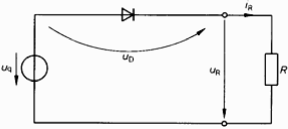
\includegraphics[height=1.2cm]{bilder/EinwegGleichrichtung.png}
            	\end{minipage} &
            		\begin{minipage}{4cm}
                    	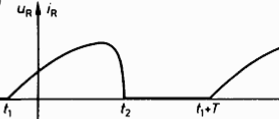
\includegraphics[width=4cm]{bilder/AusgangsspannungStromEinwegGleichrichtung.png}
                    \end{minipage} &
					\begin{minipage}{8cm}
                    	Fliesst nur ein Strom in Durchlassrichtung der Diode. \\
                    	Summe der Oberwellen $i_0=0.2176A$ \\
                    	$t_1 < t < t_2$ $\Rightarrow$ $u_R = u_q$ ; $i_R = u_q/R$ ; $u_D = 0$ \\
                    	$t_2 < t < (t_1+T)$ $\Rightarrow$ $u_R = 0$ ; $i_R = 0$ ; $u_D = u_q$
                    \end{minipage} \\
				\begin{minipage}{4cm}
                	\textbf{Zweiweggleichrichtung} \\
                	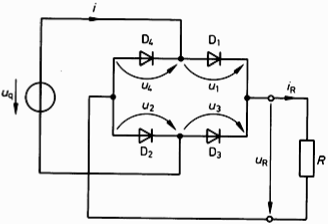
\includegraphics[height=1.5cm]{bilder/BrueckenGleichrichtung.png}
                \end{minipage} &
					\begin{minipage}{4cm}
                    	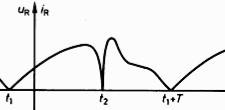
\includegraphics[width=4cm]{bilder/AusgangsspannungBrueckenGleichrichtung.png}
                    \end{minipage} &
					\begin{minipage}{9cm}
                    	Ausgangsspannung ist Betrag der Eingangsspannung. \\
                    	$t_1 < t < t_2$ $\Rightarrow$ $D_1,D_2$ leiten ; $D_3,D_4$ sperren \\
                    	$t_2 < t < (t_1+T)$ $\Rightarrow$ $D_1,D_2$ sperren ; $D_3,D_4$ leiten \\
                    	$u_R = |u_q|$ ; $i_R = u_R/R = |i|$
                    \end{minipage}
            \end{tabular}
	\subsection{Sinusf\"ormige Schwingungen von Spannung und Strom}
 		\subsubsection{Erzeugung sinusf\"ormiger Schwingungen}
 			\begin{minipage}{6cm}
 				\textbf{Lenzsche Regel}\\
 					Der induzierte Strom wirkt seiner Ursache entgegen.\\
 					Ursache des induzierten Stromes ist die \"Anderung des Flusses.
             \end{minipage}
             \hfill
 			\begin{minipage}{4.5cm}
 				\textbf{Bewegte Leiter im \\ homogenen Magnetfeld}\\
             	$U = B \cdot l \cdot v_q$ \\
             	$v_q = v \cdot cos\beta = v \cdot sin\alpha$\\
        		$U = \hat{U} \cdot sin \alpha$
             \end{minipage}
 			\begin{minipage}{3.5cm}
             	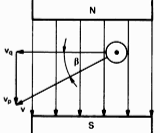
\includegraphics[width=3.5cm]{bilder/BewegteLeiter.png}
             \end{minipage}
 			\begin{minipage}{3.5cm}
             	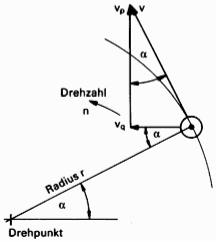
\includegraphics[width=3.5cm]{bilder/KreisfoermigeBewegung.png}
             \end{minipage}
% 		\subsubsection{Beschreibung sinusf\"ormiger Spannungen und Str\"ome}
% 			\begin{tabular}{p{6cm}p{4.5cm}p{7.5cm}}
%             	\textbf{Kreisfrequenz} &
%             		\fbox{$\omega = \frac{2 \pi}{T} = 2 \pi f$} &
%             		$[\omega] = s^{-1}$ \\ \\
%             	\textbf{Effektivwert für sinusf\"ormige Gr\"ossen} &
%             		\fbox{$U = \frac{\hat{u}}{\sqrt{2}} \quad I = \frac{\hat{i}}{\sqrt{2}}$}
%             \end{tabular}
\subsubsection{Komplexe Zeiger}
	\begin{minipage}[t]{6cm}
	  	\textbf{Prinzip der Zeigertechnik}
    \end{minipage}
	\begin{minipage}{6cm}
       	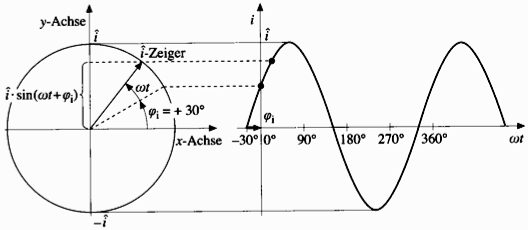
\includegraphics[width=6cm]{bilder/RotierenderScheitelwertzeiger.png}
    \end{minipage}
	\begin{minipage}{3.5cm}
       	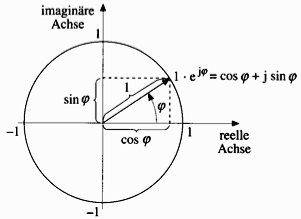
\includegraphics[width=3.5cm]{bilder/EulerscheRelation.png}
    \end{minipage} \\
	\begin{tabular}{p{4.0cm}p{5.5cm}p{8.5cm}}
       	Komplexer Effektivwert &
       		$\underline{U} = \frac{\underline{\hat{u}}}{\sqrt{2}}$ &
       		$\underline{U}$ = Kompl. Effektivwert, $\underline{\hat{u}}$ = Kompl. Scheitelwert \\
			Exponentialform &
			$\underline{\hat{u}} = \hat{u} \cdot e^{j\varphi_u} \quad \underline{U} = U \cdot e^{j\varphi_U}$  &
			$\varphi_U$ = Nullphasenwinkel der Spannung\\
			Algebraische Form &
			$\underline{\hat{u}} = \hat{u} (\cos(\varphi_u)+j\sin(\varphi_u))$ &
			$\Real(\underline{\hat{u}}) = \hat{u} \cdot \cos(\varphi_u)$ \quad $\Imag(\underline{\hat{u}}) = \hat{u} \cdot \sin(\varphi_u)$ \\
			&	$\underline{U} = U (\cos(\varphi_U)+j\sin(\varphi_U))$ &
			$\Real(\underline{U}) = U \cdot \cos(\varphi_U)$ \quad $\Imag(\underline{U}) = U \cdot \sin(\varphi_U)$ \\
			Umrechnung &
			$|\hat{u}| = \sqrt{\Real(\underline{\hat{u}})^2 + \Imag(\underline{\hat{u}})^2}$ \break $\varphi_u = \arctan\left(\dfrac{\Imag(\underline{\hat{u}})}{\Real(\underline{\hat{u}})}\right)$ \\
			&	$|U| = \sqrt{\Real(\underline{U})^2 + 		\Imag(\underline{U})^2}$ \break
			$\varphi_u = \arctan\left(\dfrac{\Imag(\underline{U})}{\Real(\underline{U})}\right)$ \\
			Komplexe Drehzeiger & 	
			\multicolumn{2}{l}{$\underline{u}(t) = \underline{\hat{u}} \cdot e^{j\omega t} = \hat{u} \cdot e^{j\varphi_u} \cdot e^{j\omega t} = \hat{u} \cdot e^{j(\omega t + \varphi_u})$} \\
			Phasenwinkel & 
			$\varphi = \varphi_u - \varphi_i$ &
			$\varphi > 0$: $U$ eilt $I$ vor\\ 
			& 	$\varphi = \frac{\Delta t}{T}\cdot 2\pi$ &
			$\varphi < 0$: $U$ eilt $I$ nach\\
		\end{tabular}
	\subsubsection{Komponenten linearer Wechselstromnetzwerke}% \formelbuch{125}}
			\begin{tabular}{llll}
			$\underline{Z} = R +j X$: 
				& Komplexer Widerstand (Impedanz); 
				& $R$: Wirkwiderstand (Resistanz); 
				& $X$: Blindwiderstand (Reaktanz)\\
			$\underline{Y} = G + j B$: 
				& Komplexer Leitwert (Admittanz); 
				& $G$: Wirkleitwert (Konduktanz); 
				& $B$: Blindleitwert (Suszeptanz)
	      	\end{tabular} \\ \\
			\begin{tabular}{|l|l|l|l|l|l|ll|}
			\hline
				\textbf{Widerstand} & 
					\multicolumn{2}{l|}{$ \underline{Z}_R = R$} & \multicolumn{2}{l|}{$ \underline{Y}_R = G =\frac{1}{R}$} &
					&
					\parbox[c][0.8cm][c]{1cm}{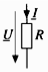
\includegraphics[height=1cm,angle=90]{bilder/Wirkwiderstand.png}}&
                	\parbox[c][0.8cm][c]{1cm}{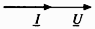
\includegraphics[width=1cm]{bilder/WirkwiderstandZeiger.png}} \\
			\hline	                    
				\textbf{Induktivität} &
					$ \underline{Z}_L = j \omega L = j X_L$&
					$ X_L = \omega L$ &
					$ \underline{Y}_L = \frac{1}{j \omega L} = j B_L$ & 
					$ B_L = - \frac{1}{\omega L}$ &
					$ W_L=\frac12 L {I_L}^2$  &
					
		            \parbox[c][0.8cm][c]{1cm}{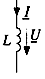
\includegraphics[height=1cm,angle=90]{bilder/Spule.png}}&
		            \parbox[c][1cm][c]{1cm}{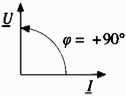
\includegraphics[width=1cm]{bilder/SpuleZeiger.png}}
		            \\
			\hline		                
				\textbf{Kondensator} &
					$ \underline{Z}_C = \frac{1}{j \omega C} = jX_C $ &
					$ X_C = - \frac{1}{\omega C} $ &
					$ \underline{Y}_C = j \omega C = j B_C $&
					$ B_C = \omega C $ &
					$ W_C=\frac12 C {U_C}^2$ & 
		            \parbox[c][0.8cm][c]{0.8cm}{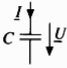
\includegraphics[height=0.9cm,angle=90]{bilder/Kondensator.png}}&
		            \parbox[c][1cm][c]{1cm}{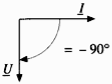
\includegraphics[width=1cm]{bilder/KondensatorZeiger.png}}\\
			\hline	    
				\parbox[c][1cm][c]{2cm}{}&
					\multicolumn{2}{l|}
						{$ \underline{Z} = \frac{\underline{U}}{\underline{I}} = \frac{\underline{U}^2}{\underline{S}^*} = 
							\frac{\underline{S}}{\underline{I}^2} $} &
					\multicolumn{2}{l|}
					{$ \underline{Y} = \frac{\underline{I}}{\underline{U}} = \frac{1}{\underline{Z}} $} &
					&
					& \\
			\hline       
			\end{tabular}
	%	\subsubsection{Berechnung linearer Wechselstromnetzwerke}
		\renewcommand{\arraystretch}{2}
		\subsubsection{Leistung im Wechselstromnetzwerk}% \formelbuch{162}}
				\begin{tabular}{p{4cm}p{7cm}p{7cm}}
					\multirow{2}{4cm}{Komplexe Leistung}  &
						$ \underline{S} = P + jQ$  & \textbf{TR:}\\
						& $ \underline{S} = \underline{U} \cdot \underline{I}^\ast = U\cdot I \cdot e^{j(\varphi_u-\varphi_i)} = \frac{\underline{U}^2}{n\underline{Z}^*} = \underline{I}^2 \cdot \underline{Z}$ & $u(t)\cdot \texttt{conj } i(t)$ 
						\\
					Scheinleistung [VA]	& $ S = U\cdot I = \frac{U^2}{Z} 
						= I^2 \cdot Z = \sqrt{P^2+Q^2}$& \\
					Wirkleistung [W] &
						$ P = \Real(\underline{S}) = S \cos(\varphi) = I^2 \cdot \Real(\underline{Z}) $ \\
					Blindleistung [var] &
						$ Q = \Imag(\underline{S}) = S \sin(\varphi)  = P \cdot
						\tan\left(\varphi\right)$ & Kapazitiv: $Q < 0$; induktiv: $Q > 0$ \\
					Leistungsfaktor &
						$\lambda = \frac{P}{S} = \frac{P}{U\cdot I} = \underbrace{\cos \varphi}_{\text{bei sinus Schwingungen}}$ \\
				\end{tabular}
		\renewcommand{\arraystretch}{1}
		\input{idiotenseite/elektrotechnik/subsections/ohmscheLeistung}
		\subsubsection{Blindleistungskompensation (mit Kondensator)}
\renewcommand{\arraystretch}{1.5}
\begin{tabular}{p{7cm}p{4.5cm}p{5cm}}
	Kompensation mit C &
    	\begin{minipage}{4cm}
        	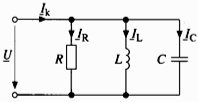
\includegraphics[width=3.5cm]{bilder/Parallelkompensation.png}
        \end{minipage} & 
		Der Kondensator wird parallel dazu geschalten \\ \\
	Zeigerdiagramme Kompensation &
		\begin{minipage}{4.5cm}
        	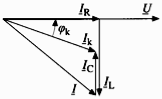
\includegraphics[width=3.5cm]{bilder/Blindstromkompensation.png}
        \end{minipage} &
		\begin{minipage}{4.5cm}
        	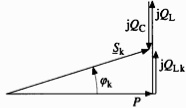
\includegraphics[width=3.5cm]{bilder/Blindleistungskompensation.png}
        \end{minipage} \\ \\
	Neue (kompensierte) Blindleistung &
		$Q_{Lk} = P \cdot \tan{\varphi_k}$ \\
	Blindleistung des Kondensators & 
		\multicolumn{2}{l}{$Q_C = Q_{Lk} - Q_L =  P\cdot (\tan{\varphi_k}-\tan{\varphi}) $} \\
	Kapazität des Kondensators &
		$C = - \frac{Q_C}{\omega U^2}$ \\	
	\end{tabular}
\renewcommand{\arraystretch}{1}

	\begin{minipage}{0.49\textwidth}
		\subsubsection{Serieschaltung von $R_S$ \& $X_S$}
		\begin{tabular}{lll}
		%		& $Z = R_S + jX_S$ &\\
		%		& $\varphi = \arctan(\frac{X_S}{R_S})$ & \\
		%		& $U_R = U_0 \cdot \cos\varphi $& \\
		%		& $U_X = U_0 \cdot \sin\varphi $ & \\
		%		& $P = \frac{U_R^2}{R_S} = I^2\cdot R_S$ &\\
		%		& $Q = \frac{U_X^2}{X_S} = I^2\cdot X_S$&
		\end{tabular}
		\begin{align*} 
			Z 		&	= R_S + jX_S 				  \\
			\varphi &	= \arctan(\frac{X_S}{R_S}) 	  \\
			U_R 	&	= U_0 \cdot \cos\varphi 	  \\
			U_X		&	= U_0 \cdot \sin\varphi 	  \\
			P		&	= \frac{{U_R}^2}{R_S} = {I_0}^2\cdot R_S  \\
			Q		&	= \frac{{U_X}^2}{X_S} = {I_0}^2\cdot X_S					
		\end{align*}
	\end{minipage}
	\begin{minipage}{0.49\textwidth}
	\subsubsection{Parallelschaltung von $R_P$ \& $X_P$}
	\begin{align*}
		Z 		&	= \frac{1}{\frac{1}{R_P}+j(-\frac{1}{X_P})}	\\
		\varphi &	= \arctan(- \frac{R_P}{X_P})				\\
		I_R 	&	= I_0 \cdot \cos\varphi						\\
		I_X		&	= I_0 \cdot \sin\varphi						\\
		P		&	= \frac{{U_0}^2}{R_P} = {I_R}^2\cdot R_P	    \\
		Q		&	= \frac{{U_0}^2}{X_P} = {I_X}^2\cdot X_P
	\end{align*}
	\end{minipage}
	
		

		\subsubsection{Leistungsumsatz bei nichtsinusf\"ormigen periodischen Gr\"ossen}
		\begin{minipage}[c]{7.5cm}
			\parbox{4cm}{Allgemein: Indizes beziehen sich auf Harmonische (Bsp: 0. Har = DC)\\}
			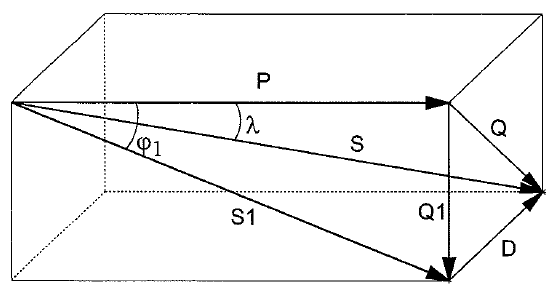
\includegraphics[height=4cm]{bilder/ZeigerdiagrammNichtSinus.png}     
    	\end{minipage}%
		\begin{minipage}[c]{10.5cm}   
    		\noindent
    		\renewcommand{\arraystretch}{2.0}
    		\begin{tabular}{|p{3.6cm}p{7.3cm}|}
	    		\hline
	        		Unterwelle: 
	        			& $X_{U} = \overline{X} = \hat{X}\dfrac{a_0}{2}  \qquad $  \\
	        	\hline
		     		Grundwelle: 
		     			& $X_{G} = \dfrac{\hat{X}}{\sqrt{2}} \sqrt{a_1^2 + b_1^2} \qquad  $   \\
		     	\hline
		     		Oberwellen: 
		     			& $X_{O} = \dfrac{\hat{X}}{\sqrt{2}}
		     			\sqrt{\sum\limits_{k=2}^{\infty}a_k^2 +\sum\limits_{k=2}^{\infty}b_k^2}
		     			\qquad $  \\ 
		     	\hline
		     		Effektivwerte:&
		     		 $X_{RMS} = \sqrt{X_G^2 + X_O^2}$ \newline  $X_{TRMS} =
		     			\sqrt{X_U^2 + X_{RMS}^2}$ \\
	     		\hline
					ges. Blindleistung: &
						$Q = 	\sqrt{Q_G^2 + Q_U^2 + U^2  \sum\limits_{k=2}^{\infty}{I_k^2}} = \sqrt{Q_1^2 + D^2}$ \\
				\hline 
					Grundschwinungs-Blindleistung: &
						$Q_1 = \sqrt{{S_1}^2 - P^2}$ \\
				\hline
					Wirkleistung: &
						Durch Signale gleicher Frequenz umgesetzt, $P_R = {I_{TRMS}}^2 \cdot R$ \\
				\hline
					Verzerrungsblindleistung: &
						$D = U \cdot \sqrt{I_{\mu}^2 + \sum\limits_{k=2}^{\infty}I_k^2}$ \\
				\hline
					Grundschwinungs-Scheinleistung: &
						$S_1 = U \cdot I_G$ \\
				\hline
					ges. Scheinleistung: &
						$S = \sqrt{P^2 + {Q_1}^2 + D^2} = U \cdot I_{TRMS}$ \\
				\hline
		 	\end{tabular} \\
		 \renewcommand{\arraystretch}{1}
     	\end{minipage}    		\\ \\
     	Die Verzerrungsblindleistung wird von den Oberwellen und ev. von der Unterwelle (je
     	nach Phasenverschiebung) verursacht und ist mit Kondensatoren \textbf{nicht} zu kompensieren -
     	Aktive Filter w\"aren n\"otig.
		\\		
		
	\begin{minipage}[c]{8cm} 
	   \textbf{Beispiel anhand eines Einweggleichrichters:}	  	\\
	   (mit ohmscher Last R) 
	\end{minipage}   
	\begin{minipage}[c]{10cm} 	
	   $ \qquad i_d(t) = \underbrace{\frac{\hat{I}}{\pi}}_{Unterwelle} + \underbrace{\frac{\hat{I}}{2}
	   \sin(\omega t)}_{Grundwelle} - \underbrace{\frac{2\hat{I}}{\pi} \sum\limits_{k=1}^n \frac{1}{(2k-1)(2k+1)} \cos(2k\omega t)}_{Oberwellen} $
	\end{minipage}   
		
	\begin{minipage}[c]{10cm}  
		\begin{tabular}{| l | l | l |}
    		\hline 
      		\textbf{Bezeichnung}
      		& \textbf{rel. Wert$^\ast$}
      		& \textbf{Formel} ($I_s = I_d$)\\
      		\hline
      		Scheitelwert
      		& $\hat{I} = \sqrt{2} = 1,414$
      		& $= \hat{I}_d = \frac{\hat{U}_d}{R} $ \\
      		Mittelwert (DC)
      		& $I_U = 0.45$
      		& $= I_m = \bar{I}_d = \frac{\hat{I}}{\pi}$ \\
      		Grundwelle
      		& $I_G = 0.5$
      		& $= \frac{\hat{I} \cdot \sqrt{2}}{\pi}$ \\
      		Oberwellen
      		& $I_O = 0.2162$
      		& $= \hat{I} \cdot \sqrt{2} \cdot 0.21762$ \\
      		Effektivwert (AC)
      		& $I_{_{RMS}} = 0.5433$
      		& $ = \sqrt{I_G^2 + I_O^2}$\\
      		Laststrom
      		& $I_{_{TRMS}} = 0.7071$
      		& $= I_{d} = \frac{\hat{I}_d}{2} =\frac{\hat{U}_d}{2 R}$ \\
      		Primärstrom
      		&
      		& $I_1 \approx \bar{I}_d \cdot \frac{1.21}{"u}$ \\
      		Bauleistung 
      		&
      		& $S_{TR} = \frac{S_{1Tr} + S_{2Tr}}{2}$ \\
      		\cline{2-3}
			Leistungen
		 	& \multicolumn{2}{l|}{ $Q = D \qquad S_1 = P \qquad Q_1 = 0$} \\
      		\hline 
    	\end{tabular} \newline
    	$^\ast$: bezogen auf $I_{Eff} = 1A$ im AC-Stromkreis ohne Diode
	\end{minipage}   
	\begin{minipage}[c]{8cm}  
			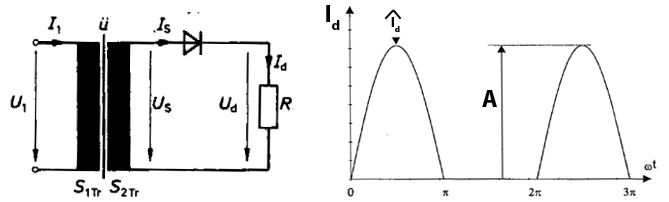
\includegraphics[width=8cm]{bilder/EinwegGR.png}  \\			
	$S_{1Tr} < S_{2Tr}$ da der Trafo keine Gleichstr\"ome übertr\"agt. Somit erscheint der Prim\"arstrom
	als Sekund\"arstrom mit unterdrücktem Gleichstromanteil.\\			
	\end{minipage}

	\begin{minipage}[c]{8cm} 
	   \textbf{Beispiel anhand eines Brückengleichrichters:}	  	\\
	   (mit ohmscher Last R)
	\end{minipage}   
	\begin{minipage}[c]{10cm} 	
	   $ \qquad i_d(t) = \underbrace{\frac{2 \hat{I}}{\pi}}_{Unterwelle} - \underbrace{\frac{4\hat{I}}{\pi} \sum\limits_{k=1}^n \frac{1}{(2k-1)(2k+1)} \cos(2k\omega t)}_{Oberwellen} $
	\end{minipage}\\
\begin{minipage}[c]{10cm}  
		\begin{tabular}{| l | l |}
    		\hline 
      		\textbf{Bezeichnung}
      		%& \textbf{N\"aherungsformel}
      		& \textbf{Formel} \\
      		\hline
      		Scheitelwert 
      		%& %& $\hat{I} = 0.7071 \cdot A $
      		& $\hat{I} = \hat{I}_d = \frac{\hat{U}_d}{R} $ \\
   %   		Fourien-Reihe
    %  		&$i(t)=A(\frac{2}{\pi}-\frac{4}{\pi}(\frac{\cos(2t)}{1\cdot
 %     		3}+\ldots+\frac{\cos(2nt)}{(2n-1) \cdot (2n+1)}))$\\
      		Unterwelle (Mittelwert)
      		%& $I_U = 0.22508 \cdot A $
      		& $I_U = \bar{I}_d = \frac{2 \hat{I}}{\pi}$ \\
      		Grundwelle
      		%& $I_G = 0.25 \cdot A$ 
      		& $I_G = 0$ \\
      		Oberwellen
      		%& $I_O = 0.10881 \cdot A$ 
      		& $I_O = \frac{\hat{I}}{\sqrt{2}} \cdot 0.43524$ \\
      		%Effektivwert (RMS)
      		%& $I_{RMS} = 0.27265 \cdot A$
      		%& $I_{RMS} = \sqrt{I_G^2 + I_O^2}$ \\ 
      		Laststrom
      		%& $I_{TRMS} = 0.35355 \cdot A$
      		& $I_{d} = I_{TRMS} =  \frac{U_s}{R}= \frac{\hat{U}_d}{\sqrt{2}R}$ \\ 
      		Diodenstrom
      		& $I_{V} = \frac{\hat{U}}{2 R} = \frac{I_{d}}{\sqrt{2}}$ \\
      		Prim\"arstrom
      		& $I_1 \approx \bar{I}_d \cdot \frac{0.966}{"u}$ \\
      	%	Bauleistung 
      	%	& $S_{TR} = \frac{S_{1Tr} + S_{2Tr}}{2}$ \\
      	 	\hline
    	\end{tabular}
	\end{minipage}   
	\begin{minipage}[c]{8cm}  
			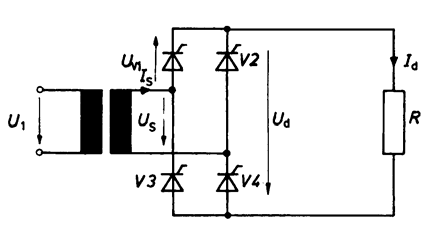
\includegraphics[width=7cm]{bilder/brueckengleichrichter.png}  \\			
	$S_{1Tr} < S_{2Tr}$ da der Trafo keine Gleichstr\"ome übertr\"agt. Somit erscheint der Prim\"arstrom
	als Sekund\"arstrom mit unterdrücktem Gleichstromanteil.			
	\end{minipage}
